\begin{filecontents*}{u28_refs.bib}
@article{abadie2006,
  author = {Abadie, Alberto and Imbens, Guido W.},
  title = {Large Sample Properties of Matching Estimators for Average Treatment Effects},
  journal = {Econometrica},
  year = {2006},
  volume = {74},
  number = {1},
  pages = {235--267}
}

@article{angrist1996,
  author = {Angrist, Joshua D. and Imbens, Guido W. and Rubin, Donald B.},
  title = {Identification of Causal Effects Using Instrumental Variables},
  journal = {Journal of the American Statistical Association},
  year = {1996},
  volume = {91},
  number = {434},
  pages = {444--455}
}

@book{imbens2015,
  author = {Imbens, Guido W. and Rubin, Donald B.},
  title = {Causal Inference for Statistics, Social, and Biomedical Sciences},
  publisher = {Cambridge University Press},
  year = {2015}
}
\end{filecontents*}

\documentclass[10pt]{article}
\usepackage[margin=0.82in]{geometry}
\usepackage[T1]{fontenc}
\usepackage{lmodern}
\usepackage{amsmath}
\usepackage{amsthm}
\usepackage{array}
\usepackage{booktabs}
\usepackage{tabularx}
\usepackage{graphicx}
\usepackage{subcaption}
\usepackage{tikz}
\usetikzlibrary{arrows.meta,calc,positioning,shapes.geometric}
\usepackage[round,authoryear]{natbib}
\usepackage[colorlinks=true,linkcolor=blue,citecolor=blue,urlcolor=blue]{hyperref}
\usepackage[nameinlink,noabbrev]{cleveref}

\newtheorem{theorem}{Theorem}
\crefname{theorem}{theorem}{theorems}
\Crefname{theorem}{Theorem}{Theorems}

\title{Integrated Conversion Stress Paper}
\author{Stage Two Corpus}
\date{}

\begin{document}
\maketitle

\begin{abstract}
This paper combines common scholarly structures that frequently appear together in applied research manuscripts. The example includes linked floats, mathematical displays, theorem statements, footnotes, author-year citation commands rendered through \texttt{natbib}, and an appendix. The substantive topic is a small observational evaluation in which site-level decisions are summarized through tables and diagrams. The fixture is dense by design, because conversion failures often arise when otherwise ordinary features interact in the same document.
\end{abstract}

\section{Introduction}

Applied evaluation papers routinely mix prose, mathematical definitions, diagnostics, and tables. The conversion problem becomes difficult when these elements are cross-referenced throughout the text, because a local formatting decision can change how readers find the evidence. In the present example, \cref{fig:workflow} gives the design logic, \cref{fig:subdiagnostics} reports two diagnostic panels, and \cref{tab:regression} presents the main numerical result.

The notation follows the potential-outcomes framework described by \citet{imbens2015}. Matching estimators are used as a compact reference point because their finite-sample behavior is familiar and well documented \citep{abadie2006}. The instrument notation in \cref{eq:target} follows the convention in \citet{angrist1996}, although the example remains descriptive rather than a claim about a real intervention.\footnote{The data in this fixture are synthetic and are included only to test document conversion behavior.}

\section{Design and Estimands}

Let $i$ index units, $s(i)$ index sites, and $Z_i$ denote assignment to a screening recommendation. The observed outcome is written as
\begin{align}
Y_i &= Z_iY_i(1) + (1-Z_i)Y_i(0), \label{eq:observed}\\
X_i &= \left(1,\; \mathrm{risk}_i,\; \mathrm{load}_{s(i)},\; \mathrm{prior}_{s(i)}\right)^{\top}, \\
\hat{m}_z(x) &= \frac{1}{|\mathcal{N}_z(x)|}\sum_{j\in\mathcal{N}_z(x)} Y_j .
\end{align}
The target contrast averages site-specific differences with weights proportional to baseline volume:
\begin{equation}
\tau = \sum_{s=1}^{S}\omega_s\left\{E[Y_i(1)\mid s(i)=s]-E[Y_i(0)\mid s(i)=s]\right\}, \qquad \sum_{s=1}^{S}\omega_s=1.
\label{eq:target}
\end{equation}
The block in \cref{eq:observed} and the scalar target in \cref{eq:target} are separated to test both aligned equations and ordinary numbered equations.

\begin{theorem}[Stable weighted aggregation]
\label{thm:aggregation}
Suppose each site-level contrast $\tau_s$ is bounded by $M$ in absolute value and the estimated weights $\hat{\omega}_s$ satisfy $\sum_s|\hat{\omega}_s-\omega_s|\leq \eta$. Then the aggregation error induced by replacing $\omega_s$ with $\hat{\omega}_s$ is at most $M\eta$.
\end{theorem}

\begin{proof}
The difference between the two weighted averages is
\[
\left|\sum_s(\hat{\omega}_s-\omega_s)\tau_s\right|.
\]
Applying the triangle inequality and the uniform bound $|\tau_s|\leq M$ gives the stated upper bound. The result is used only as a formatting fixture, yet it also gives a simple check on the notation in \cref{eq:target}.
\end{proof}

\section{Workflow and Diagnostics}

\begin{figure}[tbp]
\centering
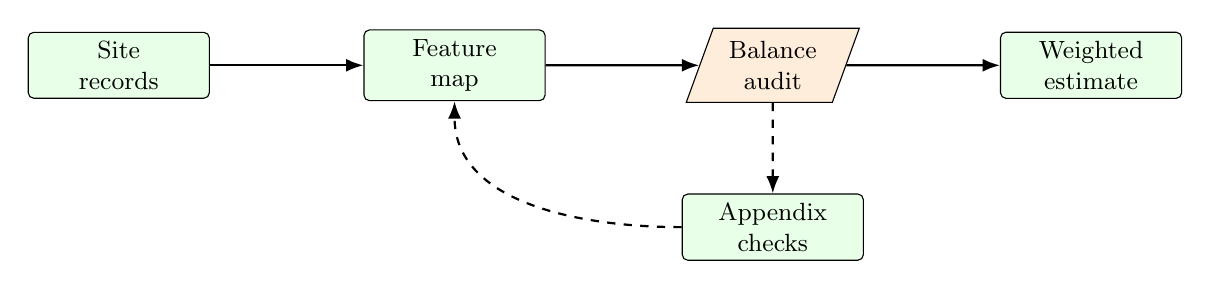
\begin{tikzpicture}[
  node distance=1.95cm,
  every node/.style={font=\small},
  stage/.style={draw, rounded corners=2pt, align=center, minimum width=2.3cm, minimum height=0.72cm, fill=green!9},
  audit/.style={draw, trapezium, trapezium left angle=70, trapezium right angle=110, align=center, minimum width=2.2cm, fill=orange!14},
  arrow/.style={-{Latex[length=2.2mm]}, thick}
]
\node[stage] (records) {Site\\records};
\node[stage, right=of records] (features) {Feature\\map};
\node[audit, right=of features] (audit) {Balance\\audit};
\node[stage, right=of audit] (estimate) {Weighted\\estimate};
\node[stage, below=1.15cm of audit] (appendix) {Appendix\\checks};
\draw[arrow] (records) -- (features);
\draw[arrow] (features) -- (audit);
\draw[arrow] (audit) -- (estimate);
\draw[arrow, dashed] (audit) -- (appendix);
\draw[arrow, dashed] (appendix.west) to[out=180,in=-90] (features.south);
\end{tikzpicture}
\caption{Analysis workflow represented as a TikZ diagram.}
\label{fig:workflow}
\end{figure}

\Cref{fig:workflow} is a compact representation of the evaluation process. It deliberately mixes ordinary rectangular nodes with a trapezium audit node and a feedback arrow, because these shapes probe a converter's treatment of TikZ geometry.

\begin{figure}[tbp]
\centering
\begin{subfigure}[t]{0.47\linewidth}
\centering
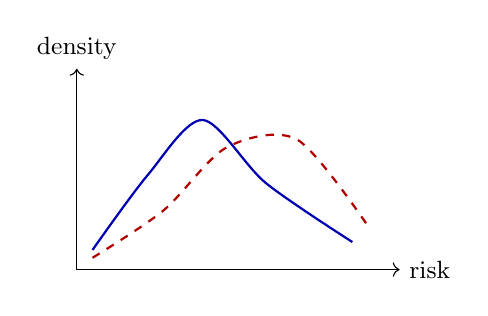
\begin{tikzpicture}
\draw[->] (0,0) -- (4.1,0) node[right] {\small risk};
\draw[->] (0,0) -- (0,2.55) node[above] {\small density};
\draw[blue!70!black, thick] plot[smooth] coordinates {(0.2,0.25) (0.9,1.2) (1.6,1.9) (2.4,1.1) (3.5,0.35)};
\draw[red!70!black, thick, dashed] plot[smooth] coordinates {(0.2,0.15) (1.1,0.75) (1.9,1.55) (2.8,1.65) (3.7,0.55)};
\end{tikzpicture}
\caption{Score density}
\label{fig:sub-density}
\end{subfigure}
\hfill
\begin{subfigure}[t]{0.47\linewidth}
\centering
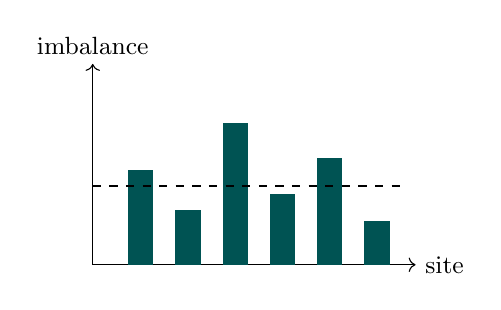
\begin{tikzpicture}
\draw[->] (0,0) -- (4.1,0) node[right] {\small site};
\draw[->] (0,0) -- (0,2.55) node[above] {\small imbalance};
\foreach \x/\h in {0.45/1.2,1.05/0.7,1.65/1.8,2.25/0.9,2.85/1.35,3.45/0.55}{
  \fill[teal!65!black] (\x,0) rectangle +(0.32,\h);
}
\draw[dashed] (0,1) -- (3.95,1);
\end{tikzpicture}
\caption{Site imbalance}
\label{fig:sub-imbalance}
\end{subfigure}
\caption{Subfigure diagnostics for the synthetic evaluation.}
\label{fig:subdiagnostics}
\end{figure}

The subfigures in \cref{fig:subdiagnostics} contain separate captions and labels, allowing references to \cref{fig:sub-density} and \cref{fig:sub-imbalance} as individual panels. This arrangement is a common source of numbering and caption placement errors.

\section{Results}

\begin{table}[tbp]
\centering
\caption{Regression-style summary of synthetic estimates}
\label{tab:regression}
\begin{tabular}{@{}lccc@{}}
\toprule
 & Baseline & Site adjusted & Matched \\
\midrule
Recommendation effect & 0.142 & 0.118 & 0.104 \\
 & (0.031) & (0.029) & (0.027) \\
Risk score & 0.284 & 0.241 & 0.229 \\
 & (0.044) & (0.041) & (0.039) \\
Prior volume & 0.017 & 0.012 & 0.010 \\
 & (0.006) & (0.005) & (0.005) \\
\midrule
Site fixed effects & No & Yes & Yes \\
Matched controls & No & No & Yes \\
Observations & 1,280 & 1,280 & 1,112 \\
\bottomrule
\end{tabular}
\end{table}

\begin{table}[tbp]
\centering
\caption{Tabularx audit matrix with paragraph cells}
\label{tab:audit}
\begin{tabularx}{\linewidth}{@{}lXcc@{}}
\toprule
Check & Description & Threshold & Status \\
\midrule
Overlap & Compares empirical score support between recommendation groups after trimming the outer two percent of observations. & $0.08$ & Pass \\
Missingness & Computes site-specific missingness in the core feature vector and flags cells with $m_s>0.10$. & $0.10$ & Review \\
Influence & Re-estimates \cref{eq:target} after removing one site at a time and records the largest absolute shift. & $0.03$ & Pass \\
\bottomrule
\end{tabularx}
\end{table}

The coefficient pattern in \cref{tab:regression} is consistent with attenuation after adjustment, and the audit matrix in \cref{tab:audit} records the supporting diagnostics in paragraph-style cells. Taken together with \cref{thm:aggregation}, these objects provide a compact set of references that travel across prose, equations, and floats.

\section{Robustness Interpretation}

The matched specification in \cref{tab:regression} is treated as the main summary because it uses the same target contrast defined in \cref{eq:target} while reducing the most visible score imbalance in \cref{fig:sub-density}. The interpretation remains descriptive. A reader should understand the coefficient as the difference associated with receiving a recommendation after conditioning on the observed feature vector, rather than as a fully identified causal parameter. This wording matters for conversion testing because it places a careful methodological qualification near citations, equation references, and table references in ordinary paragraph form. The paragraph also contains a second note marker for the footnote surface.\footnote{This additional note is included to test multiple footnotes in a document that also contains floats, theorem environments, and an appendix.}

The site imbalance panel in \cref{fig:sub-imbalance} motivates a second robustness check based on leave-one-site-out estimates. Let $\hat{\tau}_{(-s)}$ denote the estimate after excluding site $s$. The reported influence diagnostic is
\[
  I = \max_{1\leq s\leq S} |\hat{\tau}_{(-s)}-\hat{\tau}|.
\]
This scalar is included in \cref{tab:audit}, where the threshold is written in a paragraph cell rather than in a standard numeric column. Placing mathematical notation in a prose-heavy table cell tests whether conversion preserves the balance between inline formulas and wrapped text.

The appendix extends this robustness discussion by reporting small sensitivity calculations. Its role is deliberately modest: it creates an appendix label, an appendix float, and cross-references from the main text to material that appears after the sectioning reset. The final reference to \cref{app:checks} should therefore resolve to an appendix section, while \cref{tab:appendix-grid} should retain ordinary table numbering within the appendix context. Together these references create a practical check on how the converter handles late-document labels after BibTeX has already introduced its own auxiliary files.

\section{Discussion}

The integration fixture is meant to expose failures that appear only when features are combined. For example, the paragraph cells in \cref{tab:audit} include a live reference to \cref{eq:target}; the subfigure captions in \cref{fig:subdiagnostics} use a nested numbering scheme; and the bibliography requires a BibTeX pass generated from an embedded database. The appendix provides an additional sectioning transition so that downstream tools must preserve both main-matter and appendix labels.

\appendix

\section{Additional Checks}
\label{app:checks}

This appendix records two supplementary calculations. First, replacing the weights in \cref{eq:target} with equal weights changes the estimate from $0.104$ to $0.097$. Second, removing the site with the largest value of $\mathrm{load}_{s(i)}$ changes the estimate to $0.109$. These numbers are synthetic, but they create ordinary appendix prose with mathematical notation and cross-references.

\begin{table}[tbp]
\centering
\caption{Appendix sensitivity grid}
\label{tab:appendix-grid}
\begin{tabular}{@{}lcc@{}}
\toprule
Scenario & Estimate & Difference from matched model \\
\midrule
Equal weights & 0.097 & $-0.007$ \\
Largest site removed & 0.109 & $0.005$ \\
Borderline cases removed & 0.101 & $-0.003$ \\
\bottomrule
\end{tabular}
\end{table}

\Cref{tab:appendix-grid} is included so that the appendix contains a float of its own. The final bibliography should appear after the appendix and should resolve the \texttt{\textbackslash citep} and \texttt{\textbackslash citet} commands used in the main text.

\bibliographystyle{plainnat}
\bibliography{u28_refs}

\end{document}
